% ONLY IN CHAPTER 1

\addtocontents{toc}{\vspace{2em}} % Add a gap in the contents, for aesthetics

% Begin numeric (1,2,3...) page numbering

\pagestyle{fancy} % Return the page headers back to the "fancy" style

% Chapter 1

\chapter{Introduction} % Main chapter title

\label{chap:ntroduction} % For referencing the chapter elsewhere, use \ref{Chapter1} 

\lhead{Chapter 1. \emph{Introduction}} % This is for the header on each page - perhaps a shortened title

%----------------------------------------------------------------------------------------

\section{Graphs and graph signals}

In the field of discrete mathematics, the term ``graph" denotes a collection of distinct objects that may possess some form of pairwise connection or association. The discrete objects that make up the graph are referred to as nodes (or vertices), and their connections are known as edges (or arcs). This abstract definition can be applied to represent numerous real-world structures. For example, in an airline route map, nodes could symbolise airports, and edges could indicate the presence of a direct flight.


\begin{wrapfigure}{r}{0.4\linewidth}
	\centering
		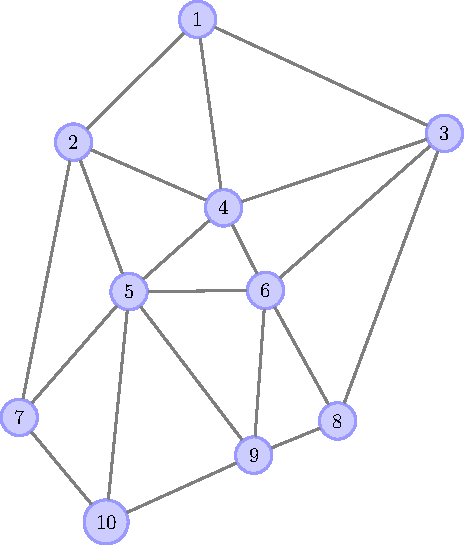
\includegraphics[width=\linewidth]{Figures/graph_plot.pdf}
	\caption[A visual representation of a simple graph]{A visual representation of a simple graph with 10 nodes and 20 edges.}
	\label{fig:basic_graph}
\end{wrapfigure}


Graphs and network models are employed in many actively researched areas of mathematics, including network processes such as epidemic modelling \citep{Pare2020}, graph neural networks \citep{Zhou2020}, graphical models \citep{Holmes2008}, and semi-supervised learning \citep{Chong2020}.

In this thesis, we focus primarily on the area of Graph Signal Processing (GSP), a rapidly evolving field that sits at the intersection of spectral graph theory, statistics, and data science \citep{Ortega2018}. GSP is devoted to the mathematical analysis of signals that are defined over the nodes of a graph, simply referred to as \textit{graph signals}. \phantom{In this thesis we are  }

\begin{wrapfigure}{l}{0.4\linewidth}
	\centering
		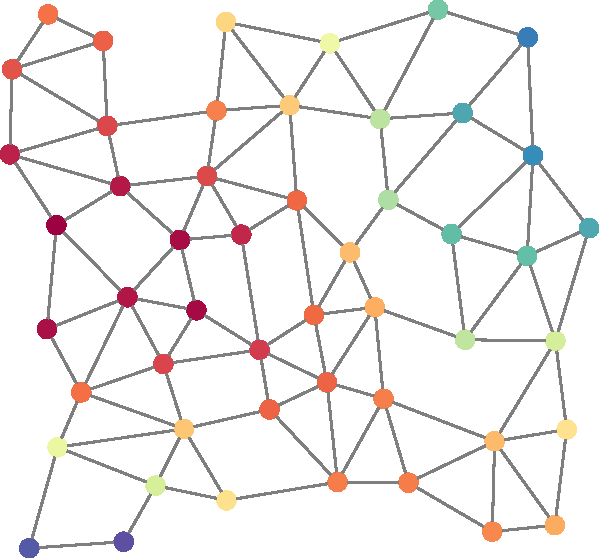
\includegraphics[width=\linewidth]{Figures/graph_signal_plot.pdf}
	\caption[A graphical depiction of a graph signal]{A graphical depiction of a graph signal. Here, the value of the signal at each node is represented by its color.}
	\label{fig:graph_signal}
\end{wrapfigure}
 

A graph signal represents a value that is measured simultaneously at every node in a graph. For example, consider a social media network, where each node represents an individual, and presence of an edge indicates that the two individuals have connected. An example of a graph signal in this context could be the age of each person in the network, or a score indicating their propensity to engage with certain content. In either case, this is a value that could theoretically be measured or estimated across the network, though it may be subject to missing data or noise. 

GSP typically uses tools that stem from classical signal processing. There, the focus is on manipulating data that resides on a regular domain, such as audio, images and digital communication. GSP utilises spectral graph theory to generalise these classical techniques, leading to graph-based counterparts of algorithms such as filtering, sampling, and reconstruction \citep{Sandryhaila2013}. Applications of GSP are numerous, ranging from social networks \citep{Dong2015} and brain connectivity modelling \citep{Huang2016} to sensor networks \citep{Zhu2012}, and molecular structures \citep{Kearnes2016}. As an emerging field, there are many opportunities for the development of theory, and new use-cases to explore, making it an exciting and dynamic area of research. 

The primary focus of this thesis is on statistical models for the estimation of noisy, partially observed multivariate graph signals. In particular, we formulate several Bayesian regression and reconstruction models designed for multivariate data, and investigate scalable approaches to solving them in practice. This begins, in \cref{chap:gsr_2d}, with the reconstruction of signals with two axes, such as network time series data. \Cref{chap:kgr_rnc_2d} introduces several regression techniques for two-dimensional graph signals, and \cref{chap:nd_gsp} generalises the techniques developed prior in the thesis to $d$-dimensional data, under the ``MultiWay" GSP (MWGSP) framework. This is followed, in \cref{chap:variance}, by an investigation into the posterior covariance of the models, and finally \cref{chap:binary} introduces generalisations for binary and categorical graph signals. Along the way, there are several methodological contributions as well as some detailed case studies. In this introductory chapter, we first establish some basic definitions and concepts from GSP, as well as highlighting some motivating use cases. In \cref{chap:lit_review}, we define the precise scope of this thesis, review the relevant literature, and present our core contributions. 


\section{GSP fundamentals}

A graph, $\mathcal{G}$, with $N$ vertices is described by a node set $\mathcal{V}$, and an edge set $\mathcal{E}$. In this thesis, we will be primarily concerned with undirected graphs without self-loops, meaning the edges have no preferential direction and nodes do not connect to themselves. By imposing some arbitrary but consistent ordering on the nodes, this graph can also be described by an $N \times N$ adjacency matrix $\A$, where the entry $\A_{ij} = \A_{ji} \geq 0$ holds the strength of connection between nodes $i$ and $j$. In the basic case of a non-weighted graph, $\A_{ij}$ is simply one if the corresponding edge exists and zero otherwise. Using the same ordering, a graph signal can be represented by a vector, $\y$, of length $N$, where $\y_i$ holds the value of the graph signal at node $i$. 

One key property of a graph signal is its \textit{smoothness}. Intuitively speaking, a smooth graph signal should exhibit gentle variation between closely connected nodes, as is the case in \cref{fig:graph_signal}. Conversely, a rough graph signal might see large jumps in signal value between neighbouring nodes. Mathematically, the smoothness of a signal, $\y$, defined over the nodes of an undirected graph, can be measured in several ways. One simple option is the total square variation ($\text{TV}_2$), defined as follows. 

\begin{equation}
    \label{eq:TSV1}
    \text{TV}_2(\y) = \frac{1}{2}\sum_{i=1}^N \sum_{j=1}^N \A_{ij} (\y_i - \y_j)^2
\end{equation}

This metric sums up the square difference in signal value at each neighbouring node, weighted by the corresponding entry in the adjacency matrix, with the factor of a half adjusting for the double counting of nodes. It can also be written in terms of a single quadratic form, by introducing a new matrix $\LL$ - the so-called graph \textit{Laplacian}. 

\begin{equation}
    \label{eq:TSV2}
    \text{TV}_2(\y) = \y^\top \LL \y
\end{equation}

The Laplacian, like the adjacency matrix $\A$, is another symmetric $N \times N$ matrix, and is defined as $\LL = \D - \A$, where $\D$ is the degree matrix. $\D$ is a diagonal operator, where entry $\D_{ii}$ holds the sum of all the edge weights linked to node $i$, or in other words, the vector along the diagonal of $\D$ is the column (or row) sum of $\A$. The Laplacian, which can be interpreted as a generalisation of the discrete second order derivative operator for an irregular topology, is of central importance to many aspects of GSP \citep{Shuman2013}. 

\newpage

It is straightforward to show that the two expressions for the total square variation given in \cref{eq:TSV1,eq:TSV2} are equivalent, see for example chapter 3 of \cite{Ortega2022}. A few basic facts stand out about the Laplacian quadratic form.

\begin{enumerate}
    \item $\y^\top \LL \y \geq 0$ for any $\y$. Since $\text{TV}_2(\y)$ sums the square difference between the signal at each pair of nodes, weighted by the non-negative entries of the adjacency matrix, the Laplacian quadratic form must be strictly non-negative. By definition, this implies that the matrix $\LL$ is positive semi-definite (PSD). 
    \item $\one^\top \LL \one = 0$, where $\one$ is a length-$N$ vector of ones. If the signal of interest is constant over the whole graph, the total square variation must be zero. Furthermore, if the graph contains two or more isolated sub-graphs, with edges connecting nodes within a each group but not between groups, then any signal that is constant over each sub-graph will have a Laplacian quadratic form of zero. 
\end{enumerate}

Since $\LL$ is positive semi-definite, its eigenvalues are all real and non-negative, and its eigenvectors can be chosen to be real and orthonormal. Thus, $\LL$ can be decomposed as follows. 

\begin{equation}
    \LL = \U \LAM \U^\top
\end{equation}

where $\U$ is the orthogonal, $N \times N$ matrix of eigenvectors $\{\uu_i\}$, and $\LAM$ is the diagonal matrix of corresponding eigenvalues $\{\lambda_i\}$, typically given in ascending order. Since $\U$ is orthonormal, it holds that $\uu_i^\top \uu_j = \delta_{ij}$, and that $\{\uu_i\}$ form a set spanning $\R^N$. Given the definition of the Laplacian quadratic form, the eigenvectors are the unique set of orthonormal vectors that sequentially minimise the total square variation, subject to perpendicularity to all those previous \citep{Spielman2019}. 


$$
\begin{matrix}
    \uu_1 & = & \underset{\raisebox{-0.1cm} { $ \scriptstyle |\uu|^2 = 1$ }}{\text{argmin}} \quad & \text{TV}_2(\uu) \\[0.7cm]
    \uu_2 & = & \underset{\raisebox{-0.1cm} { $ \scriptstyle |\uu|^2 = 1, \; \perp \uu_1$ }}{\text{argmin}} \quad & \text{TV}_2(\uu) \\[0.7cm]
    \uu_3 & = & \underset{\raisebox{-0.1cm} { $ \scriptstyle |\uu|^2 = 1, \;\perp \uu_1, \uu_2$ }}{\text{argmin}} \quad & \text{TV}_2(\uu) \\[0.7cm]
    \uu_4 & = & \ldots
\end{matrix}
$$

\newpage

In this way, the eigenvectors of the graph Laplacian can be understood as sequentially less and less smooth, with respect to the topology of the graph. The corresponding eigenvalue, referred to as the frequency, gives a value specifying how ``rough'' each eigenvector is relative to the others, as measured by $\text{TV}_2$. Note that, for any undirected graph, the first Laplacian eigenvector will always be constant with an eigenvalue of zero. \Cref{fig:uk_eigs} gives a visual depiction of the first eight Laplacian eigenvectors and eigenvalues for a network representing local authority regions in the UK. \footnote{Using boundary data published by the Office for National Statistics \citep{ONS2019}}  

\begin{figure}[t]
	\centering
		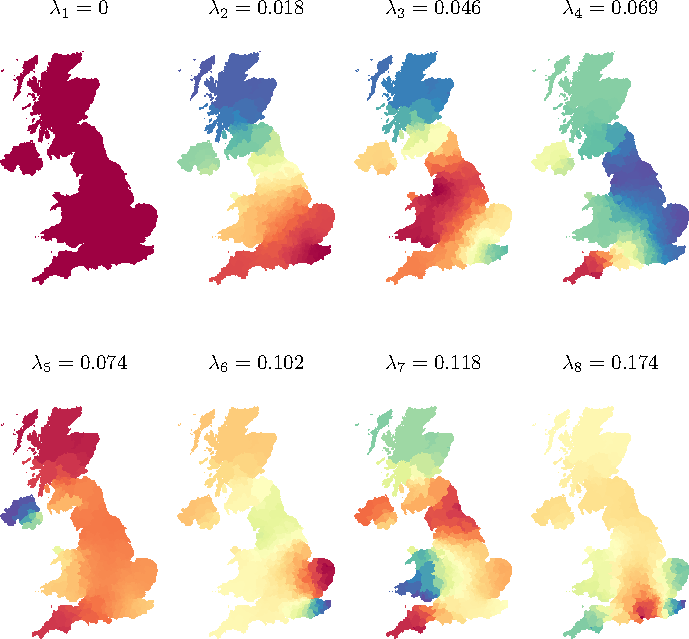
\includegraphics[width=0.85\linewidth]{Figures/uk_plot.pdf}
		% \rule{35em}{0.5pt}
        \caption[A visualisation of the Laplacian eigenvectors for a network of regions in the UK]{A visualisation of the first eight Laplacian eigenvectors, along with their associated eigenvalue, for a network of local authority regions in the UK. Each node represents a region, and each pair of regions share an edge if they border one another (or have a direct ferry crossing). Again, color is used to represent the value of the the graph signal. }
	\label{fig:uk_eigs}
\end{figure}


Since $\{\uu_i\}$ span the total space of $\R^N$, any graph signal, $\y$, can be decomposed into a weighted sum of the Laplacian eigenvectors. This parallels the classical Fourier transform, which expands signals into the basis of complex exponentials \citep{Sneddon1995}. As such, any graph signal, $\y$, has a duel representation, $\z$, in the frequency domain. Transformations between these two representations can be achieved by applying the Graph Fourier Transform (GFT) and Inverse Graph Fourier Transform (IGFT), which amounts to multiplying by the matrices $\U^\top$ and $\U$ respectively. 

\begin{align}
    \z &= \mkern 2mu \text{GFT}(\y) \mkern 2mu = \U^\top \y \\[0.2cm]
    \y &= \text{IGFT}(\z)  = \U \z
\end{align}

For some simple graphs, the GFT is equivalent to a well-known transform in classical signal processing. For example, the Laplacian of the cycle graph (i.e. a set of nodes connected in a loop) has eigenvectors that can be expressed as sines and cosines (or, in full generality, complex exponentials) \citep{Puschel2003}. \Cref{fig:cycle_eighs} gives a visualisation of the real eigenvectors of a 50-node cycle graph Laplacian. 

\begin{figure}[t]
	\centering
		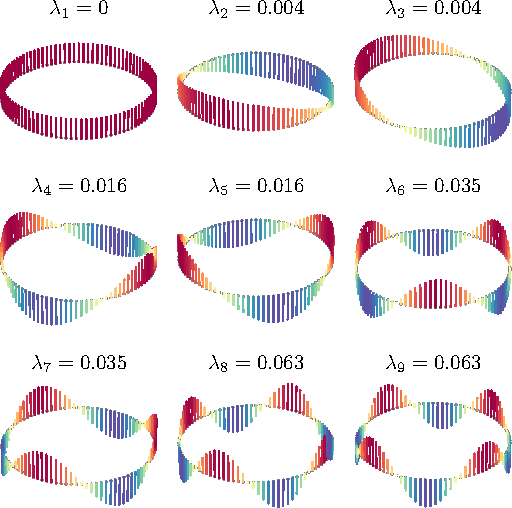
\includegraphics[width=0.65\linewidth]{Figures/loop_plot.pdf}
        \caption[A visualisation of the real Laplacian eigenvectors of the cycle graph]{A visualisation of the first nine Laplacian eigenvectors of a cycle graph with 50 nodes, along with their associated eigenvalue.}
	\label{fig:cycle_eighs}
\end{figure}

Given that any graph signal can be decomposed into its Laplacian frequency components, filters and other spectral operators can be defined quite naturally. First, take a signal $\y$ and transform it into the frequency domain via the GFT. Next, scale each frequency component according to some predetermined function. Finally, transform back into the node domain via the IGFT. 


\begin{wraptable}{l}{0.5\linewidth}
    \centering
    \def\arraystretch{1.7}
    \begin{tabular}{@{}l c@{}}
        \toprule
        \textbf{Filter}   & $g(\lambda; \,\beta)$   \\
        \midrule
        1-hop random walk & $(1 + \beta \lambda)^{-1}$ \\
        Diffusion         & $\exp(-\beta \lambda)$\\
        ReLu              & $\max (1 - \beta \lambda, 0)$\\
        Sigmoid           & $2 \big( 1 + \exp(\beta \lambda)\big)^{-1}$\\
        Bandlimited       & $1, \,\text{if} \; \beta \lambda \leq 1 \; \text{else} \; 0$ \\
        \bottomrule
       \end{tabular}
       \caption[Example graph filter functions]{Some example graph filter functions}
        \label{tab:filters}
\end{wraptable}

A low-pass filter is a spectral operator that attenuates high-frequency components from a graph signal \citep{Ricaud2019}. It can be described by a monotonically decreasing filter function, $g(\lambda)$, which maps a Laplacian frequency, $\lambda$, to a number ranging between one and zero. The filtered signal, $\y'$, can then be computed as follows. 


\begin{equation}
    \y' \, =\U \mkern 2mu g(\LAM) \mkern 2mu \U^\top = \, \HH \y
\end{equation}


$g(\LAM)$ is the diagonal matrix found by applying the function $g$ to each entry along the diagonal of $\LAM$, and $\HH = \U g(\LAM) \U^\top$ is the resultant positive semi-definite graph filter operator \citep{Isufi2022}. \Cref{tab:filters} gives some example filter functions, which also depend on a positive scalar parameter $\beta$ controlling the intensity of the filtering operation. Larger values of $\beta$ correspond to more aggressive attenuation of the high frequency content. In the limit as $\beta \rightarrow \infty$, these filters retain only the constant component, and as $\beta \rightarrow 0$, all frequency components are allowed through the filter unaffected. 

Graph filters can also be constructed in other ways. One notable example is using finite order polynomials. The benefit of polynomial filters is that their action on a graph signal can be computed by repeated application of the Laplacian, meaning $O(N^3)$ eigendecomposition can be avoided. An order-$P$ polynomial filter $g(\lambda) = \sum^P a_p \lambda^p$ can be applied to a graph signal as follows \citep{Susnjara2015}. 

\begin{equation}
    \U \mkern 2mu g(\LAM) \mkern 2mu \U^\top \y = \big(a_0 \I_N + a_1 \LL + a_2 \LL^2 + ... + a_P \LL^P \mkern 2mu \big) \, \y
\end{equation}

If the Laplacian is sparse, or has special structure, repeated multiplications of $\y$ by $\LL$ can computed with complexity $ < O(N^2)$. Furthermore, the computation is ``local'' in the sense that element $i$ of the filtered signal can be computed using data no more than $P$ hops away via graph edges. For this reason, polynomial filters lend themselves well to distributed GSP applications, such as a network of sensors that communicate locally in the vertex domain. \Cref{fig:filters_plot} gives a visualisation of the filter functions given in \cref{tab:filters}, and a polynomial filter. 

\begin{figure}[t]
	\centering
		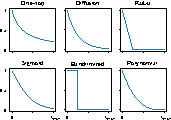
\includegraphics[width=0.7\linewidth]{Figures/filters_plot.pdf}
        \caption[The frequency response of some simple graphs filters]{The frequency response of several simple graph filters is shown. }
	\label{fig:filters_plot}
\end{figure}


% Another closely related concept is that of graph kernels. In the context of GSP, graph kernels should not be confused with another topic sharing the same name that concerns distance metrics between pairs of graphs \citep{Kriege2020}. 

% \begin{wrapfigure}{r}{0.4\linewidth}
% 	\centering
% 		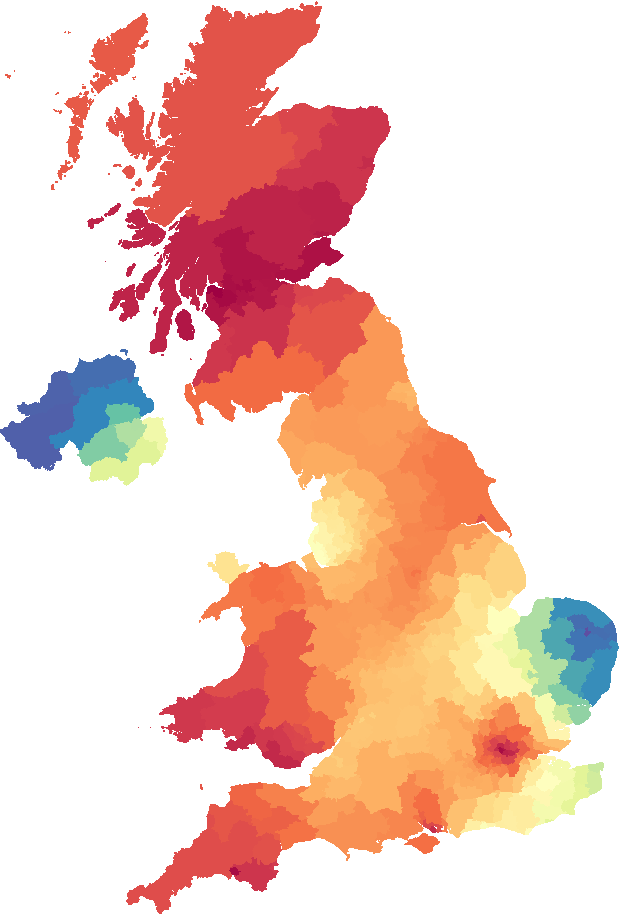
\includegraphics[width=0.75\linewidth]{Figures/uk_smooth.pdf}
% 	\caption[An example of a random smooth graph signal]{An example of a random smooth signal on the UK district graph, sampled from $\Norm{\zero}{\HH^2}$ using a bandlimited filter. }
% 	\label{fig:random_smooth_uk}
% \end{wrapfigure}

% Graph filters can also be used to describe a probability distribution over possible signals. Consider an independent multivariate normal random variable $\x \sim \Norm{\zero}{\I_N}$. Applying a graph filter to a random signal $\x$ will result in a new signal, $\HH \x$, which is smoother with respect to the graph topology. This will be distributed according to $\HH \x \sim \Norm{\zero}{\HH^2}$, meaning $\HH^2$ can be interpreted as a covariance matrix with which to generate smooth, normally distributed graph signals. \Cref{fig:random_smooth_uk} gives a visual example of a random smooth signal, drawn from a distribution constructed from a bandlimited filter, allowing only the first ten frequency components through. 


\newpage

\section{GSP use cases}

Graph signal processing methods have proven effective in many real world applications. In this short section, we highlight some recent use-cases from the literature, as motivation for the content of this thesis. 

\subsection{Biology}

The world of biology provides many interesting use cases for graph signal processing methods \citep{Li2023}. One area which has garnered significant interest is in analysing protein-protein interactions. Here, the concept is to model a set of proteins as nodes in an ``interactome'', which is the network of physical molecular interactions in a particular cell. Recent work such as \cite{Colonnese2021} used GSP methods to predict new interactions between proteins, while work such as \cite{Jha2022} used graph neural networks for the same task. These models aim to automate the prediction of protein interactions, reducing the time and cost associated with experimental methods. Other work has modelled an individual protein molecule as network of residues connected to each other based on their physical distance in 3D space, with the aim of predicting its biophysical properties \citep{Srivastava2023}. 

Another area in biology that has been the subject of study via GSP methods is brain connectivity modelling. Work such as \cite{Goldsberry2017,Atasoy2016,Menoret2017,Itani2021} has found that the graph-spectral frequency profile of signals derived form fMRI imaging can provide useful insight into brain activity. In particular, these and related works have found specific Laplacian spectral profiles associated with different emotional states, task familiarity and neurological diseases. 

\subsection{Transportation and Infrastructure}

Another area in which GSP methods have been widely applied is in transportation and infrastructure applications. In \cite{Hasanzadeh2017}, the authors propose an adaptive ARMA model in the graph frequency domain for real-time traffic prediction, which was able to achieve a substantial increase in performance over non-graph-aware alternatives. The prediction of traffic was also tackled using GSP methods in \cite{Chakraborty2017}, using a technique known as trend filtering \citep{Wang2016}, and automatic incident detection using spatio-temporally denoised thresholds was applied in \citep{Chakraborty2019}. In \cite{Xiu2022}, the authors use a spatial-temporal multi-graph convolutional wavelet network to predict passenger numbers on a metro system. 

GSP has also been used to analyse patterns of power consumption in electricity grids \citep{Ramakrishna2021}, and pressure in hydraulic networks \citep{Zhou2022}. In \cite{He2018} and \cite{Zheng2022}, the authors use GSP to address non-intrusive load disaggregation, which is an active area of research in the field of smart grids and energy conservation where the goal is to estimate how much each appliance or electrical load contributes to the total consumption. In \cite{Ying2022}, the authors address the recovery of harmonic data lost during power transmission, based on the spectral graph theory, and in \cite{Wang2022b}, the authors use GSP to identify abnormal batteries from cell-level voltage signals in a network of electric bicycle charging stations. 


\subsection{Finance and Economics}

Networks have been used in financial and economic models for many years \citep{Marti2021}, however, recently GSP specifically has found some interesting use-cases. In \cite{Vinicius2020}, the authors use a spectral model to learn an underlying graph structure from financial time-series data, and show that meaningful physical interpretations related to the market index factor can be extracted from this representation. In \citep{Zhang2023}, the authors consider how GSP can be incorporated into momentum-based financial forecasting models, showing that the additional topological information can enhance the accuracy of such models. Graph Neural Networks have also been used extensively in financial applications \citep{Wang2022c}. 

GSP has also recently been used in the context of asset allocation and portfolio theory. The portfolio cut paradigm, introduced in \citep{Dees2020}, is a graph-theoretic portfolio partitioning technique that allows the investor to group economically meaningful clusters of assets. In \citep{Arroyo2022}, this is extended by considering a dynamic portfolio, with time-evolving clusters. 



\subsection{Sensor networks}

Sensor networks are a classic application for GSP methods, since a graph is generally straightforward to construct from the physical positioning of the devices \citep{Jablonski2017}. Many of the applications in this domain are focused on distributed algorithms, since sensors and IoT devices are naturally suited to local communication. The aims of such applications are varied, encompassing tasks like compression \citep{Zhu2012}, denoising \citep{Tay2021}, reconstruction \citep{Wang2015}, and distributed data processing \citep{Chi2022}. 

Some of the earliest work that can be classified as GSP involved applications with sensor data, for example \cite{Guestrin2004}. Here, the authors used a local basis functions to design a regression algorithm capable of fast convergence with only local communication. In \cite{Wagner2005}, the authors develop a distributed wavelet transform, and applied it to a signal compression task over a network of sensors. 

